\documentclass[final,12pt]{article}
\usepackage{graphicx}
\usepackage[letterpaper,margin=1.0in]{geometry}
\usepackage{amssymb}
\usepackage{changepage}
\usepackage{float}
\usepackage{hyperref}
\usepackage{url}
\usepackage{afterpage}
\usepackage{natbib}
\usepackage{setspace}
\usepackage{fancyhdr}
\pagestyle{fancy}
\fancyhf{}
\usepackage[latin1]{inputenc} 
\usepackage{lastpage}

\def\Student{Luis Enrique CUEVAS PICOS }
\def\Title{MASTERS THESIS PROJECT}
\def\TitleESP{(ANTEPROYECTO)}
\def\Prog{Maestria en Ciencias (F\'{i}sica) }
%\def\Dept{Departamento de Investigac\'{i}on en Fis\'{i}ca}
\def\Dept{DIFUS}
\def\Institution{Universidad de Sonora}
\def\Director{Dr. Jos\'{e} Feliciano Ben\'{i}tez Rubio}
\def\ProjectTitle{Studies of the CMS Pixel Cluster Counting luminometer using Run 3 data}
\def\ProjectTitleESP{Estudios del luminometro Pixel Cluster Counting del CMS usando datos de la corrida 3}
\def\ResearchLine{Fisica Matematica}

%%header and footer
\lhead{\Student\ / \ \Dept}
\rhead{\TitleESP}
\rfoot{Page \thepage \hspace{1pt} of \pageref{LastPage}}

%%comands
\newcommand{\SubItem}[1]{ {\setlength\itemindent{15pt} \item[-] #1} }
\newcommand{\lumi}[1]{{#1~fb$^{-1}$}}
\newcommand{\instlumi}[1]{#1$\times 10^{34}$ cm$^{-2}$s$^{-1}$}

  

%%%%%%%%%%%%%%%%%%%%%%%%%%%%%%%%%%%%%
\begin{document}
\onehalfspacing

%%%%Title Page
\begin{titlepage}
\centering
\hspace{0pt}
%\vfill
{\scshape\Large \Title \\ \TitleESP \par}
%%project revised 2021-1
  
  \vspace{1cm}
  {
    TITLE:\par
    {\bf \large \ProjectTitle  \par}
       
    \vspace{0.4cm}
    TITULO:\par
    {\bf \large \ProjectTitleESP \par}
  }
       
  \vspace{1cm}
  {
    RESEARCH LINE (LGAC): \par
    \ResearchLine \par
  }
        
  \vspace{2cm}
  {\underline{\hspace{8cm}}\par}
  {\bf \scshape \Student \par}
  {Student\par}

  \vspace{1cm}
  {\underline{\hspace{8cm}}\par}
  {\scshape \Director \par}
  {Director\par}

  \vspace{1cm}
  {\bf \Prog \par}
  {\Dept \par}
  {\Institution \par}

  \vspace{2cm}
  {\today}

\hspace{0pt}
\vfill

\end{titlepage}


%%%%% white page for print out
\shipout\null


%%%% Abstract Page
\newpage
\hspace{2pt}
\vfill

  \begin{center}
    {\Large \ProjectTitle \par}
    \vspace{1cm}
    {\itshape\textbf{Abstract}\par}
  \end{center}
  
  \vspace{1 cm}
 
  
  This  project consists on  perform an analysis and calibration of the LHC luminosity data recorded
  by the CMS experiment during the new phase starting in 2022 (Run 3) using the Pixel Cluster Counting (PCC) method.
%to develop the upgraded luminosity measurement system for Run 3 and the HL-LHC phases.
Luminosity gives a measure of how many collisions are happening in a particle accelerator  and a precise determination of this will allows us precise tests of the Standard Model and searches for new physics like dark matter and supersymmetry theories.
The PCC method is an offline technique for the calculation of instantaneous luminosity  by counting the number of pixel clusters in the detector.
The high densities of pixels of the Inner Tracker of the CMS detector gives a low hit occupancy in the sensors during the proton-proton collisions, this leads to a very linear response and small  uncertainties for the luminosity measurement.   
  \hspace{2pt}
\vfill



%%%%%% Begin the body
\newpage
\section{BACKGROUND}


The standard model (SM) of particle physics is so far the best theoretical model to describe the interaction of elementary particles mediated by three of the four fundamental forces of nature which are electromagnetic force, strong nuclear force and the weak nuclear force. The SM is divided into two categories, the bosonic sector and the fermionic sector.
The bosonic sector contains particles which mediate the fundamental forces of nature and the fermionic sector contains particles which make up all known matter in our universe.
There are three generations of fermion particles: the first generation consists of up (u) quark, down (d) quark, electron and electron neutrino, the second generation consist of charm (c) quark, strange (s) quark, muon and muon neutrino, and the third generation has the top (t) quark, bottom (b) quark, tau and tau neutrino.
The bosonic sector consists of the gauge bosons: gluon, photon, $W^{\pm}$, $Z^0$ which mediate strong nuclear force, electromagnetic force and weak nuclear force respectively.
The Higgs boson ($H$), is the last of the gauge bosons, it gives mass to the other SM particles via electroweak symmetry breaking mechanism \cite{Chatrchyan:2012xdj}.
The heavy particles ($W^{\pm}$, $Z^0$, $H$, and top) can only be produced at high energy particle colliders like the Large Hadron Collider (LHC) operating at a center-of-mass energy of 13 TeV in Geneva, Switzerland (Figure ~\ref{figure5}).
Until the 90s, existence of almost all the SM particles were confirmed except the top quark and the Higgs boson. 
These had eluded previous experiments due to difficulties in the production and reconstruction of its decay products.
The top quark was discovered in 1995 at the Tevatron collider of the Fermilab laboratory, this proton collider operated with a center-of-mass energy of 1.8 TeV until 2010.
In 2012, the ATLAS and CMS experiments, with detectors placed at two points where the proton beams collide in the LHC, announced the discovery of a new particle with a mass of 125 GeV.
This particle has been identified as the Higgs boson by measuring its properties and comparing to those predicted by the SM.


Luminosity, $L$, is a key parameter at particle colliders along with the energy available in the collision.
$L$ is one of the  main figures of merit that quantify the potential for observing new particles and measuring their properties.
The instantaneous luminosity $L(t)$ is the process-independent ratio between the rate $R(t)$ of events produced per unit time and the cross section for a given process $\sigma$: $L(t) = R(t)/\sigma$.
During Run 1 (2011-2012) LHC reached a peak instantaneous luminosity of \instlumi{0.77} and delivered an integrated luminosity of about \lumi{25} with a precision of about 2.0\% 
\footnote{1 barn is a unit of area corresponding to $10^{-24}$ cm${^2}$ and 1 femtobarn (fb) = $10^{-39}$ cm$^{2}$.
For comparison, the total Higgs production cross section is 48600 fb.}.
In the first part of Run 2 (2015-2016), the delivered luminosity has been measured to be \lumi{38.4} with an unprecedented precision of 1.3\% \cite{Sirunyan:2021qkt-corr}.
For the second part of Run 2 (2017-2018), the integrated luminosity is about \lumi{78}.
%but its precise value and uncertainty remain to be determined and is the main objective of this thesis project \cite{CMS:2018elu-corr}.
After many upgrades to the different parts of the experiment, Run 3 is restarting this year 2022.
The main objective of this thesis project is to analize the first data recorded this year and provide a preliminary result of the luminosity recorded by the CMS experiment. 

The plan of the LHC till year 2038 is to obtain datasets with up to 10 times higher values of instanteneous luminosities in the final phase,
the  High Luminosity LHC (HL-LHC), and corresponding integrated luminosities of order \lumi{3000} \cite{Dainese:3};
the most updated projected luminosity performance along the  whole  life  of  LHC/HL-LHC  machine is shown Figure~\ref{figure6}.
These final datasets will provide  precise measurements of the properties of the Higgs boson and other SM particles as shown in Fig. ~\ref{figureKappasUncs}.
This figure shows that one of the dominant uncertainties which remain to be determined is due to the luminosity measurement.



\begin{figure}[H]
  \centering
  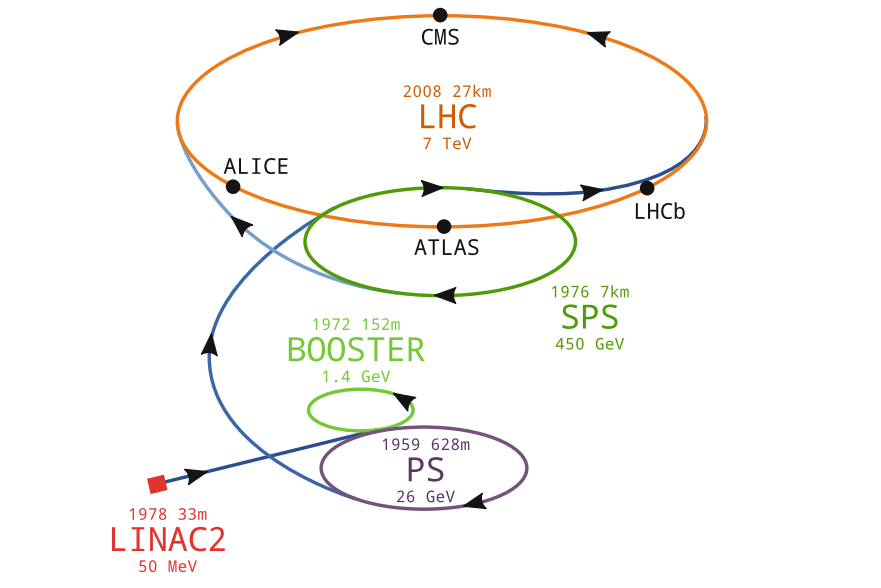
\includegraphics[width=0.7\columnwidth]{./LHC-cpx-book.png}
  \caption{Diagram of the LHC accelerator complex located near Geneva, Switzerland. The complex consists of the accelerator stages: Linear accelerator 2 (LINAC2; linear accelerator in which the protons are accelerated in bunches) , the Proton Synchrotron (PS), the Super Proton Synchrotron (SPS), and the 27 km LHC ring. Four collision points are shown corresponding to the ALICE, ATLAS, LHCb, and CMS detectors \cite{Zinser2018}.} % \cite{wiki:xxx}.} % Mobs:2684277
  \label{figure5}
\end{figure}


\begin{figure}[H]
  \centering
  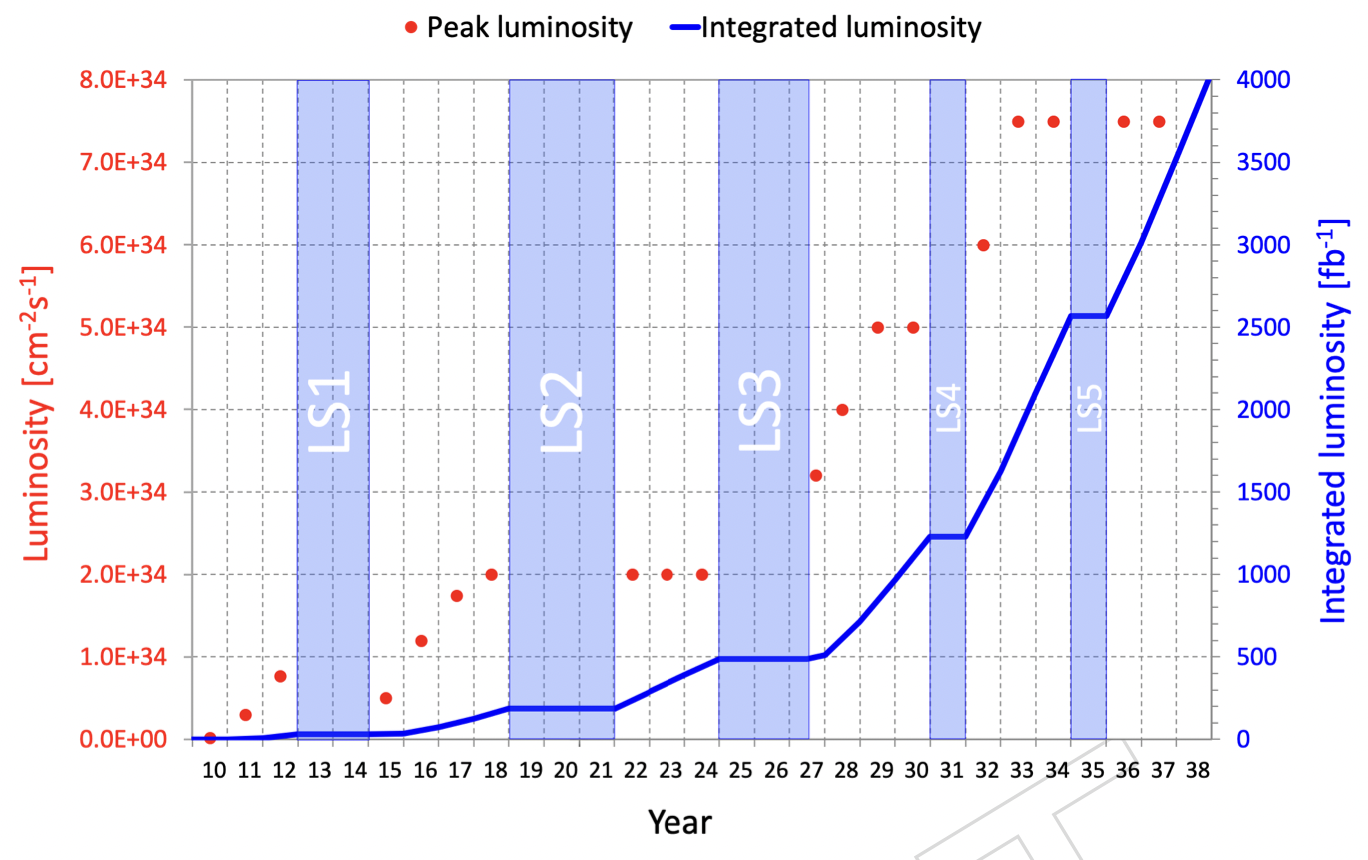
\includegraphics[width=0.8\columnwidth]{./HLLHCLumi.png}
  \caption{Forecast for peak luminosity (red dots) and integrated luminosity (violetline) in the HL-LHC era with nominal HL-LHC parameters\cite{BejarAlonso:2749422}.}  %\cite{collaborations2019report} era la [5] de la ant fig2
  \label{figure6}
\end{figure}


 \begin{figure}[H]
   \centering
   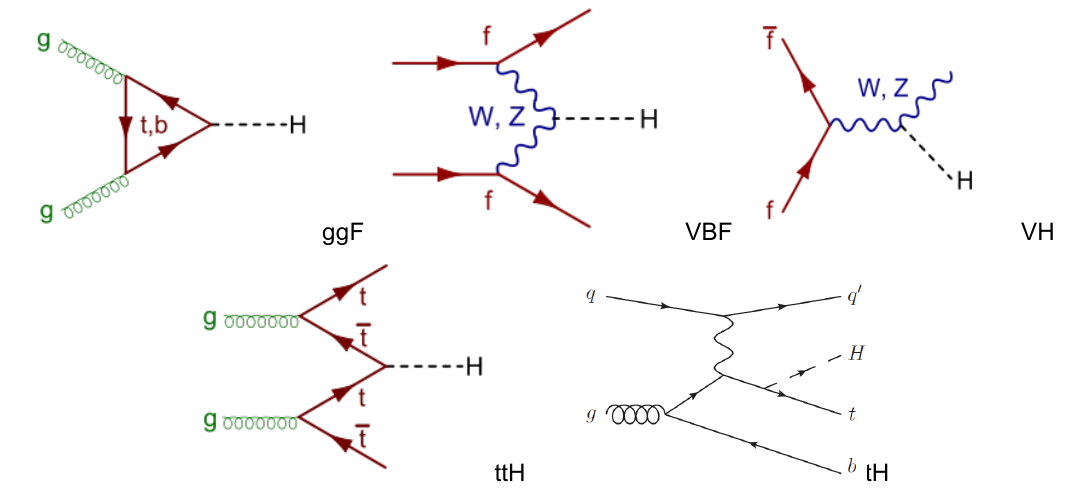
\includegraphics[width=0.6\columnwidth]{./pg.png}
   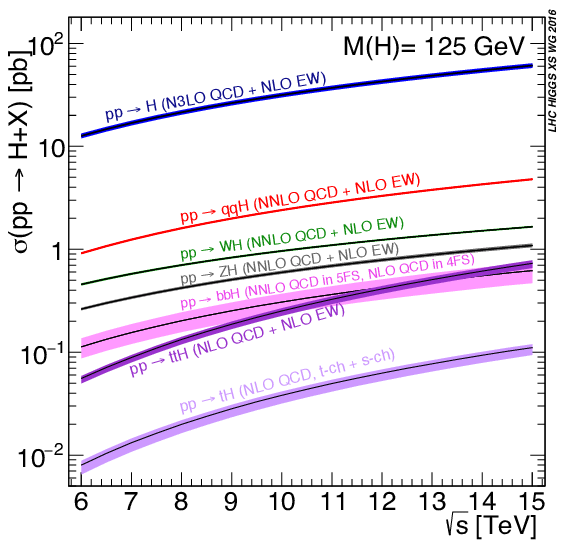
\includegraphics[width=0.39\columnwidth]{./Higgs-cross-sections-for-several-production-channels.png}
   \caption{
     Left: Main production mechanisms for the Higgs boson at the LHC: gluon-gluon fusion (ggF), vector-boson fusion (VBF), associated vector boson (VH), associated top-quark pair (ttH), and  associated single-top quark production (tH)  \cite{Grojean:2017hsb-corr}  \cite{Khachatryan:2015ota} .
     Right: Higgs boson cross sections for several production channels versus the LHC centre of mass energy  \cite{Cepeda:2019klc-corr}.
   }
   \label{figureKappasUncs}
 \end{figure}




\section{PROPOSAL}

We propose to perform an analysis and calibration of the LHC luminosity data recorded by the CMS experiment during the new phase starting in 2022 (Run 3) using the Pixel Cluster Counting (PCC) method.
In particular, we plan to perform studies of detector components and the calibration data recording using the van Der Meer (vdM) scans that allow to obtain the calibration of this luminometer with high precision.
%To develop the upgraded luminosity measurement system for Run 3 and the HL-LHC.

\section{GENERAL OBJECTIVE}

To perform an analysis and calibration of the LHC luminosity data recorded by the CMS experiment during the new phase starting in 2022 (Run 3) using the Pixel Cluster Counting (PCC) method.
%To develop the upgraded luminosity measurement system for Run 3 and the HL-LHC phases.
This will allows us precise tests of the Standard Model and searches for new physics like dark matter and supersymmetry theories.


\section{HYPOTHESIS}

For this preliminary measurement of the luminosity data collected in 2022, we expect that the methods used in this analisis will lead to a measurement uncertainty better than 2\%. 
% \cite{Dainese:3}.



\section{METHODOLOGY}

%~\ref{fig:CMS}.

The PCC method for measuring luminosity uses the Pixel detector of the CMS tracker, the layout of the  detector used for recording the data during 2016-2018 is shown in Figure~\ref{fig:pixeldet}.
The Pixel detector consists of 4 concentric cylindrical layers in the barrel and 2 disks in each endcap.
Each detector part is composed of pixel sensors, a schematic of one sensor is shown in Figure~\ref{fig:pixeldet}.
The entire Pixel detector contains 1856 sensor modules and a total of 65 million pixels.

The PCC method consists of the reconstruction of track clusters produced by charged particle tracks as shown in Figure~\ref{fig:trackcluster}.
Due to the fine granularity of the pixel sensors and the large number of total pixels, the hit occupancy in the sensors remains very small (order of 1\%) during physics runs.
This low occupancy makes the PCC  very linear as a function of pileup, an essential property of a good luminometer.

The calibration of the luminometer consists of a van der Meer (vdM) scan performed in a special LHC run usually at the beginning of the run period (year).
In this calibration setup, proton beams are moved across each other in separation steps of about 100 micrometers,
by measuring the rates of clusters with the PCC algorithm and knowledge of the beam parameters during the vdM conditions, the calibration constant ($\sigma_{vis}$) is determined.
This calibration constant is then used to normalize the measured PCC rates during normal running throughout the data-taking year \cite{pas:2018vdm}.


\begin{figure}[H]
  \centering
  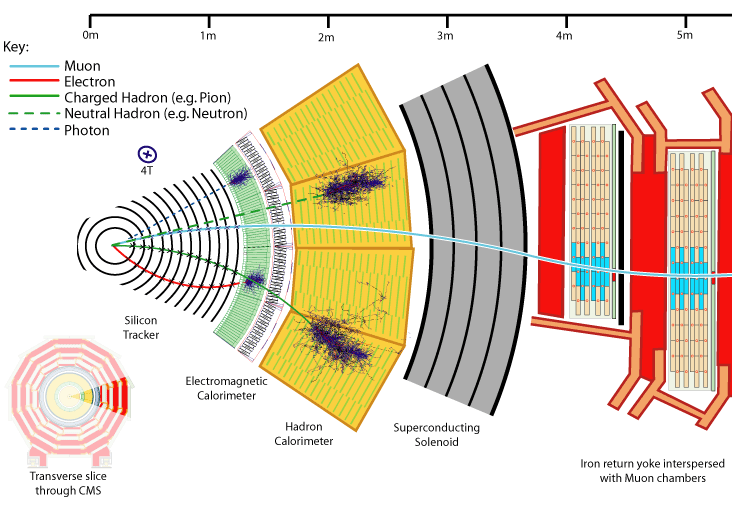
\includegraphics[width=0.7\columnwidth]{./cms_layers.png}
  \caption{Transverse view of the CMS detector showing the silicon tracker, electromagnetic calorimeter, hadron calorimeter, superconducting solenoid and muon chambers \cite{Chatrchyan:2008aa}.}
  \label{fig:CMS}
\end{figure}

\begin{figure}[H]
  \centering
  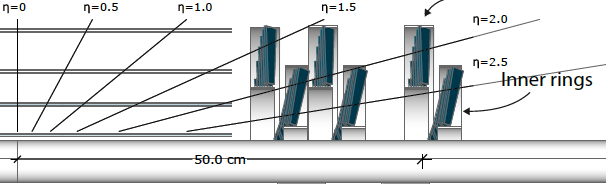
\includegraphics[width=0.7\columnwidth]{./PixelDetectorPhase1.png}
  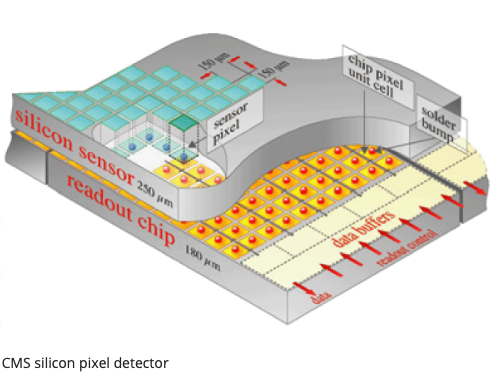
\includegraphics[width=0.27\columnwidth]{./PixelSensor.png}
  \caption{
    Left: diagram showing the layout of the CMS Pixel detector used during 2016-2018.
    The layout consists of 4 barrel layers and 2 endcap disks with two rings each.
    Right: a diagram showing the structure of one pixel sensor.
    The entire detector consists of 1856 sensors and 65 million pixels \cite{TrackerGroupoftheCMS:2020bgg}.
  }
  \label{fig:pixeldet}
\end{figure}


\begin{figure}[H]
  \centering
  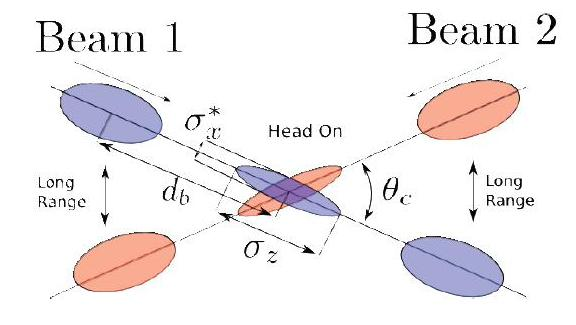
\includegraphics[width=0.5\columnwidth]{./bunchcrossing.jpg}
  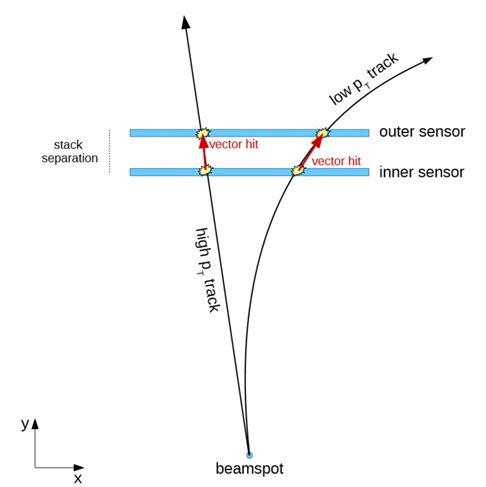
\includegraphics[width=0.4\columnwidth]{./vectorhit1.jpg}
  \caption{
    Left: Diagram showing the collision of two proton bunches at LHC, bunches contain about $10^{11}$ protons  \cite{deMaria:2008zzb}.
    Right: diagram showing example tracks originating from the collision at the beamspot and producing clusters at the pixel sensors in two detector layers.
  }
  \label{fig:trackcluster}
\end{figure}


\section{SPECIFIC OBJECTIVES}

\begin{itemize}
  
\item Understand the CMS silicon pixel detector including the barrel and endcap sensors.
  
\item Study the stability and linearity of the sensors in the different layers or disks of the pixel detector and select the stable components.
  
\item Determine new methods for measurement of the stability and linearity of the system.
  
\end{itemize}



\section{EXPECTED RESULTS}

\begin{itemize}
\item 

\end{itemize}

\section{CALENDAR OF ACTIVITIES}

\begin{itemize}

\item {\bf Summer 2021}:
  \SubItem{ Readings on Standard Model of particle physics,  the LHC and CMS experiments}
  \SubItem{ Linux/Computing skills (\textsc{Bash, Emacs, c/c++, python, ROOT})}
  \SubItem{ Computing accounts at CERN and Fermilab}
  \SubItem{ Initial planning of the analysis strategy}

\item {\bf Semester 2021-2}:
  \SubItem{ Course I: on particle physics, particle detection, or data analysis}
  \SubItem{ Analysis/Computing skills (\textsc{Bash, Emacs, c/c++, python, ROOT})}
  \SubItem{ Analysis of the LHC Run 3 luminosity data using the PCC method}

\item {\bf Semester 2022-1}:
  \SubItem{ Course II on particle physics, particle detection, or  data analysis}
  \SubItem{ Completion of the analysis of the LHC Run 3 luminosity data using the PCC method}
  \SubItem{ Presentation of results at national or international conference}
  \SubItem{ Thesis writing}

  
\end{itemize}


\onehalfspacing
\bibliographystyle{unsrt}
\bibliography{paper}

\end{document}
